\section[Opis algorytmów PIC]{Opis algorytmów PIC}\label{sec:implementation}% 20-30% - opis przyjętych rozwiązań i uzasadnienie ich wyboru
\subsection{Całkowanie równań ruchu}
Każda symulacja cząstek wymaga zastosowania integratora równań ruchu.
Tradycyjnym przykładem takiego integratora jest integrator Rungego-Kutty
czwartego rzędu, znajdujący zastosowanie w wielorakich symulacjach.

Niestety, w bieżącym kodzie nie można go zastosować ze względu na jego
niesymplektyczność: mimo ogromnej dokładności jest on niestabilny pod
względem energii cząstek\cite{computational-physics}. W symulacjach typu
Particle-in-cell konieczne jest zastosowanie innych algorytmów. Dobrym
algorytmem symplektycznym jest na przykład powszechnie znany
\emph{leapfrog}, polegający na przesunięciu prędkości o połowę iteracji
czasowej względem położeń.\cite{computational-physics} Mimo tego, że energia
układu w ruchu cząstek obliczonym tym integratorem nie jest lokalnie stała na
krótkich skalach czasowych, to jednak zachowuje energię na skali globalnej, co
pokazuje rysunek~\ref{fig:ESE-energy}. % TODO LABEL NIE DZIAŁA

\begin{figure}[h!]
  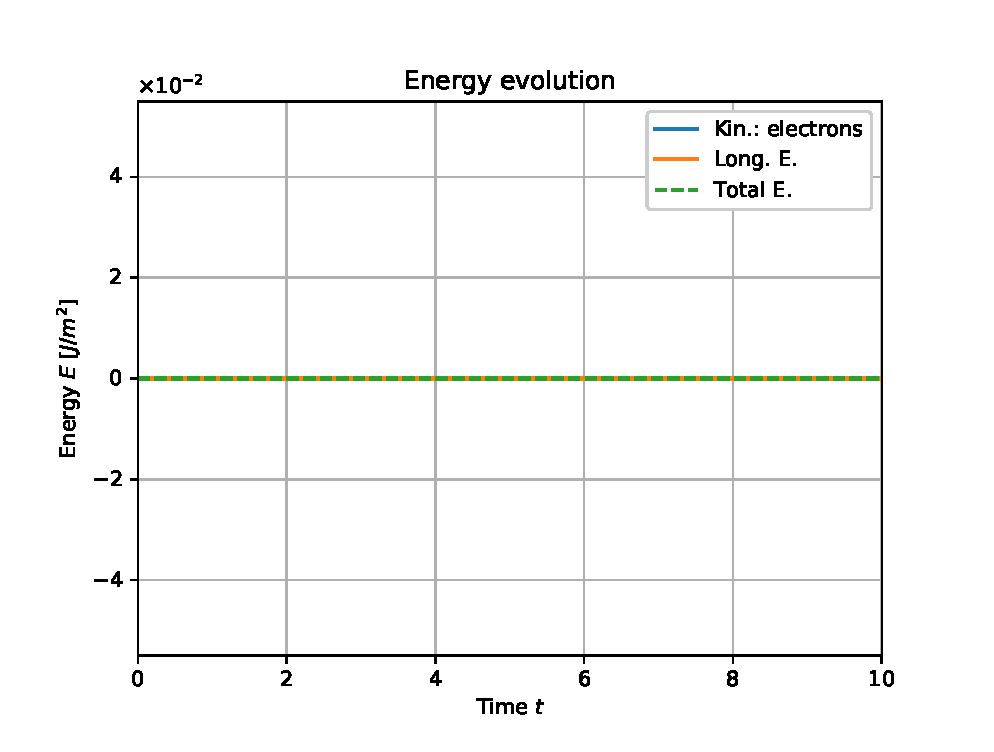
\includegraphics{Images/ESE_energy_plot}
  \caption{Energia w symulacji elektrostatycznej. Ze względu na brak pola magnetycznego
  w tej symulacji używany jest efektywnie iterator typu leapfrog.\label{fig:ESE-energy}}
\end{figure}

W przypadku ruchu w polu magnetycznym nie wystarczy, niestety, użyć
zwykłego algorytmu \emph{leapfrog}. Używa się tutaj
specjalnej adaptacji tego algorytmu na potrzeby ruchu w zmiennym polu
elektromagnetycznym, tak zwanego integratora Borysa (lepiej opisanego w~\cite{birdsall}),
który rozbija pole elektryczne na dwa impulsy,
między którymi następują dwie rotacje polem magnetycznym. Algorytm jest
dzięki temu symplektyczny i długofalowo zachowuje energię cząstek.

\begin{align}
    \vec{v}^- &= \vec{v}^{n-1/2} + \frac{q dt}{2m} \vec{E}^n 
    \label{eqn:boris-pusher-start}\\
    \vec{t} &= \frac{q dt} {2 m} \vec{B}^n \\
    \vec{v'} &= \vec{v}^- + \vec{v}^- \times \vec{t} \\
    \vec{s} &= \vec{t} / {(1 + t^2)} \\
    \vec{v}^+ &= \vec{v}^- + \vec{v'} \times \vec{s} \\
    \vec{v}^{n+1/2} &= \vec{v}^+ + \frac{q dt}{2m} \vec{E}^n \\
    \vec{x}^{n+1} &= \vec{x}^{n} + \vec{v}^{n+1/2} dt
    \label{eqn:boris-pusher-end}
\end{align}

W naszym przypadku dochodzi jeszcze jedno utrudnienie związane z
relatywistycznymi prędkościami osiąganymi przez cząstki (zwłaszcza
elektrony) w symulacji. Przed obliczeniem korekty prędkości konieczne jest
przetransformowanie prędkości z układu ``laboratoryjnego'' $\vec{v}$ na
prędkość w układzie poruszającym się z cząstką $\vec{u}$, czego dokonuje
się poprzez prostą transformację:

\begin{align}
    \vec{u} &= \vec{v} \gamma \\
    \gamma &= \sqrt{1+{(v/c)}^2} = 1/\sqrt{1+u}^2
    \label{eqn:gamma-transformation}
\end{align}


Aktualizację prędkości należy więc przeprowadzić na $\vec{u}$, nie na
$\vec{v}$. Po zakończeniu
aktualizacji należy również powrócić do $\vec{v}$ jako prędkości używanej
do depozycji prądu.

\subsection{Komunikacja między cząstkami a siatką --- depozycja i interpolacja}

Kolejnym krokiem pętli obliczeniowej po rozwiązaniu równań ruchu na
aktualizację prędkości, po której --- przypomnijmy --- dysponujemy położeniami
cząstek $x^n$ w chwilach $n$ oraz ich prędkościami $v^{n+1/2}$ w chwilach
$n+1/2$  jest obliczenie prądów podłużnych i
poprzecznych potrzebnych do obliczenia wartości pól elektromagnetycznych w
kolejnej iteracji.

W bieżącym programie gęstość ładunku jest tak naprawdę niepotrzebna w
mechanice symulacji. Ewolucja pola następuje poprzez znajomość gęstości prądu.
Jeżeli zaś pole elektromagnetyczne spełniało warunek
prawa Gaussa~\ref{eqn:maxwell-E-div} na początku, depozycja prądu w sposób
zachowujący ładunek zapewni dalsze zachowanie tego warunku w kolejnych
iteracjach.~\cite{bunemanvillasenor}

Wyjątek stanowi początek symulacji, w której pole faktycznie musi zostać
obliczone od podstaw na podstawie gęstości ładunku. \pythonpic{} pozwala
poradzić sobie z tym problemem. Pierwszą opcją jest ustawienie początkowych
położeń ładunków na identyczne między cząstkami negatywnymi i dodatnimi, co
pozwala na siłowe wyzerowanie gęstości ładunku i brak pola elektrycznego w
rejonie symulacji.

Drugą, bardziej ogólną metodą pozwalającą na niezerowy rozkład gęstości
ładunku jest zebranie gęstości ładunku z początkowych położeń cząstek i
rozwiązanie równań na pola metodą globalną (na przykład spektralnie). Jest
to jedyny moment, gdzie zebranie gęstości ładunku jest faktycznie konieczne.
Mimo to, gęstość cząstek (proporcjonalna do gęstości ładunku jako $\rho =
\sum_s q_s n_s$) jest wciąż zbierana w symulacji jako wygodna diagnostyka
ewolucji przestrzennej plazmy w obszarze symulacji. Ze względu na prostotę
algorytmu, nie zabiera ona dużo czasu obliczeniowego (do
\todo[inline]{sprawdzić dokładnie ile, rzędu 4\%}\% czasu trwania symulacji).

\subsubsection{Depozycja ładunku}

 Depozycja ładunku odbywa się w prosty sposób. Dla każdego gatunku
cząstek obliczana jest ich gęstość liczbowa (koncentracja). Najpierw
obliczane jest względne położenie każdej cząstki w komórce, do której
przynależy, poprzez
\begin{equation}
x' = (x/dx) - i_x
\label{eqn:relative-position}
\end{equation}
gdzie $i_x$ to indeks komórki, w której znajduje się cząstka.

Następnie gęstość cząstki jest rozkładana pomiędzy bieżącą komórkę a
komórkę następną w stosunku $n_i = 1-x'$, $n_{i+1} = x'$. Cząstka będąca
w połowie komórki depozytowałaby więc swój ładunek po równo między obie
komórki.

% TODO mam wrażenie że jako że tego nie wykorzystuję w symulacji to
% to może być nieco błędne, środki komórek Eulera wg depozycji ładunku są w
% połowie. Niemniej jednak, elektrostatyczne symulacje okresowe zdają się
% działać w ten sposób, nawet gdy liczę ewolucję pól poprzez prądy. To wymaga
% dalszej weryfikacji.

\begin{figure}[h!]
  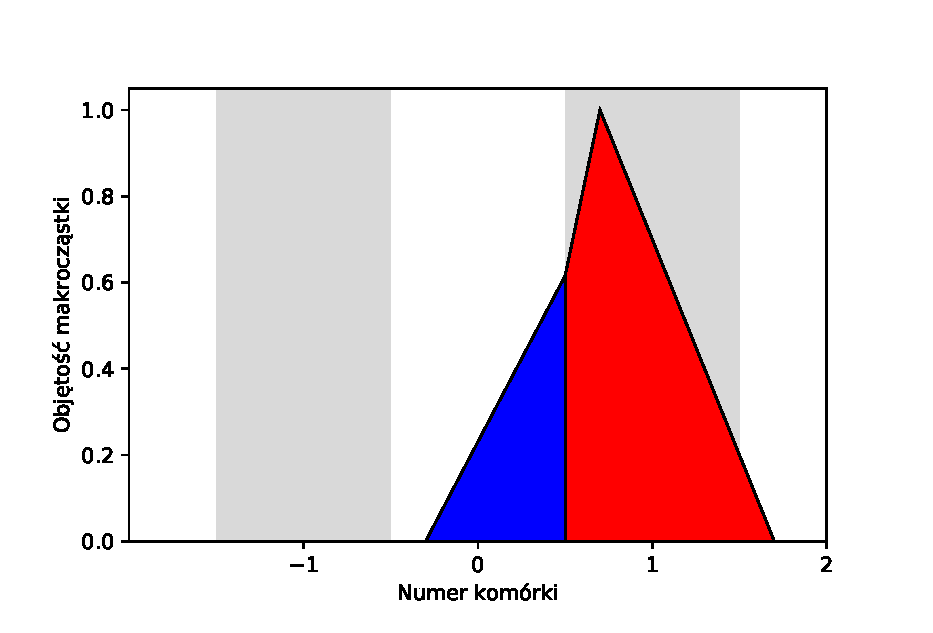
\includegraphics[width=\textwidth]{Images/charge-deposition}
  \caption{Ilustracja depozycji ładunku poprzez skalowanie pola \english{(area weighting)}.\label{fig:charge-deposition}}
\end{figure} % TODO FINISH PICTURE
\todo[inline]{Mam jakiś błąd w kodzie robiącym ten rysunek, jeszcze go oczywiście upoluję}

Po obliczeniu otrzymana tablica gęstości \emph{makrocząstek} na
siatce jest mnożona przez parametr \code{scaling} cząstek, co pozwala na
obliczenie gęstości rzeczywistych cząstek modelowanych przez makrocząstki.
Tablica gęstości ładunku jest otrzymywana poprzez zsumowanie tablic gęstości
wszystkich gatunków cząstek w układzie.

\subsubsection{Interpolacja pól elektrycznego i magnetycznego}

Interpolacja pól elektrycznego i magnetycznego odbywa się na bardzo podobnej
zasadzie, co depozycja ładunku. Wartosci pól są liniowo skalowane do pozycji
makrocząstek według ich względnych położeń (równanie~\ref{eqn:relative-position}) wewnątrz komórek.

\begin{equation}
    F = F_i (1-x') + F_{i+1} x'
    \label{eqn:field-interpolation}
\end{equation}

\subsection{Depozycja prądu} % TODO

Depozycja prądu jest bardziej złożonym zagadnieniem niż depozycja ładunku.
Prądy wymagają bowiem informacji o prędkości czastek w połówkowych
iteracjach $v^{n+1/2}$, ale sama interpolacja do komórek siatki wymaga
położeń w iteracji całkowitej $x^{n}$. Poza tym jest też kwestia, że zwykłe
liniowe przeskalowanie ładunku i parametru \code{scaling} przez prędkość w
danym kierunku nie jest wystarczające z tego powodu, że taki sposób
depozycji nie spełnia warunku zachowania ładunku.

%TODO jak sformalizować warunek zachowania ładunku
%TODO depozycja ładunku w mojej obecnej wersji nie jestem wcale przekonany że zachowuje ładunek}

To zaś dyskwalifikuje prostą liniową interpolację jako metodę depozycji
prądu, ponieważ chcemy rozwiązywać lokalne równania Ampere'a-Maxwella
zamiast liczyć globalne równania Poissona i Gaussa.
Jeżeli chcemy uniknąć obliczania poprawek korygujących dywergencję pól,
musimy to okupić większą złożonością algorytmu depozycji prądu.

Rozważamy tu zastosowany w bieżącej symulacji kształt cząstki $S_1$ (trójkątny).

Depozycja prądu jest rozbita na dwie części --- prąd podłużny i prąd
poprzeczny. Jest to spowodowane tym, że ruch w kierunkach $y$, $z$ nie
powoduje w symulacji przesuwania cząstek, a w $x$ już tak. Obliczenie prądu
w kierunkach poprzecznych jest więc jednoznaczne z obliczeniem skalowanego
\emph{przekrycia} cząstek z komórkami, przez które przechodzą w trakcie
ruchu.

Prędkość cząstek jest ograniczona przez prędkość światła, zaś za krok czasowy
przyjmujemy $\Delta t = \Delta x/c$, można więc łatwo zauważyć, że maksymalna
odległość, jaką cząstka mogłaby przebyć w jednej iteracji, to $\Delta x$.
Jeżeli cząstka wystartowałaby środkiem w lewej krawędzi komórki (swoją
własną lewą krawędzią sięgając środka poprzedniej komórki, a prawą połowy
obecnej komórki), to w czasie ruchu przemieściłaby się przez
przez łącznie trzy komórki. Ilustruje to rysunek~\ref{fig:deposition-movement}.

\begin{figure}[h!]
  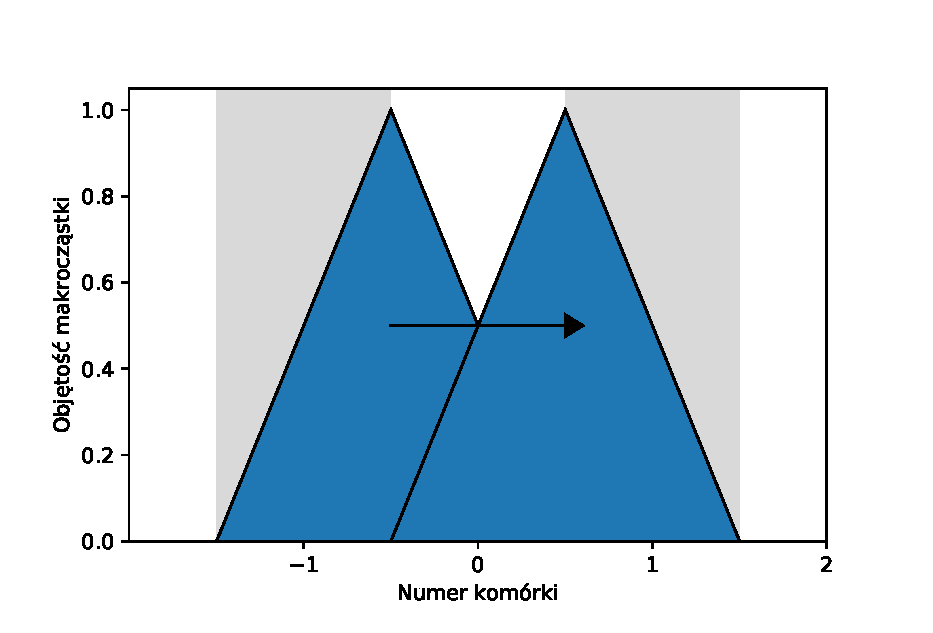
\includegraphics[width=\textwidth]{Images/deposition-movement}
  \caption{Ilustracja ruchu cząstki poruszającej się z maksymalną prędkością dozwoloną w symulacji.\label{fig:deposition-movement}}
\end{figure}

Algorytm rozbija ruch cząstek w bieżącej iteracji na etapy. W każdym z
etapów cząstka obejmuje swoim zasięgiem inne komórki. Pętla obliczeniowa
akumuluje prąd dla cząstek w następujący sposób, zaczynając z przydzielonym
czasem w bieżącej iteracji $t = \Delta t$.

\subsubsection{Depozycja podłużna} 
\begin{enumerate}
    \itemi{} obliczany jest czas potrzebny cząstce na dotarcie do kolejnej
    granicy obszaru
    \begin{equation}
        t_l = (x - x_g)/v
    \end{equation}
    Granica obszaru jest definiowana jako najbliższa połowa komórki Eulera w kierunku
    ruchu cząstki.
    \item
    \begin{itemize}
        \itemi{} jeżeli cząstka ma wystarczająco czasu $t$ (spełnia warunek $t > t_l$) aby
        dotrzeć do kolejnej granicy obszaru, jej prąd zostaje zdepozytowany przez czas $t_l$,
        \itemi{} W przeciwnym razie prąd jest depozytowany przez czas $t$ i ruch cząstki kończy się.
    \end{itemize}
    Wkład cząstki do depozytowanego prądu wynosi
    \begin{equation}
        j_x = q n v_x t/\Delta t
    \end{equation}
    \todo[inline]{Czy to jest czytelne?}
    gdzie $q$ to ładunek cząstki, a $n$ to parametr \code{scaling} oznaczający liczbę
    rzeczywistych cząstek w makrocząstce.

    \itemi{} Jeżeli ruch cząstki się nie skończył, zostaje ona (w pętli
    wewnętrznej, niezależnie od jej faktycznego ruchu w symulacji)
    %TODO właściwie możnaby zoptymalizować w ten sposób ruch cząstek, wyciąć $x += v_x \Delta t$
    przesunięta za granicę obszaru o $\varepsilon =
    10^{-10} \Delta x$. Dodanie $\varepsilon$ jest wykonywane w celu zwiększenia
    jednoznaczności porównywania liczb zmiennoprzecinkowych przy wybieraniu
    gałęzi algorytmu.

    Pętla obliczeniowa wykonuje kolejną iterację dla takiej cząstki, która tym razem
    ma przydzielony czas $t' = t - t_l$.

    Depozytowany prąd w danej iteracji trafia do komórki, w której cząstka zaczynała ruch. W ten sposób
    można zagwarantować, że cząstka zdeponuje prąd do wszystkich komórek, w których się poruszała.
\end{enumerate}

W każdej iteracji pętli obliczeniowej prąd ze wszystkich cząstek jest
akumulowany do tablicy prądów na siatce. Tablica ma rozmiar \code{NG+2} \todo[inline]{verify}

\subsubsection{Depozycja poprzeczna}
Algorytm jest identyczny do depozycji podłużnej poza samym etapem depozycji
prądu. Jako że symulacja jest jednowymiarowa i cząstki nie wykonują
faktycznego ruchu w kierunkach $y$, $z$, przyjmujemy liniową interpolację
prądów w tych kierunkach jako iloczynów $\vec{j}=q\vec{v}$ ważonych przez przekrycie
cząstki z komórkami oraz czas, jaki cząstka spędza w ruchu obejmując dane
komórki.

Przekrycie z centrum bieżącej komórki w danej chwili obliczamy jako
\begin{equation}
    s_0 = 1 \pm (x' + 0.5) 
\end{equation}
gdzie znak to $+$, gdy cząstka znajduje się w lewej połowie komórki. Zmianę
przekrycia w trakcie ruchu, jak i końcowe przekrycie, obliczamy z tym samym znakiem jako 
\begin{equation}
    s_1 = s_0 \pm \Delta s = s_0 \pm v_x t / dx
\end{equation}


Aby uzyskać wartość średniego przekrycia cząstki z komórką w trakcie ruchu
uśredniamy przekrycie na końcu ruchu z przekryciem na początku ruchu,
\begin{equation}
    w = \left(s(x^{n+1}) + s(x^n)\right)/{2}
\end{equation}

Ostatecznie wkład do bieżącej komórki w ciągu jednej iteracji pętli obliczeniowej
to $w q n v_{y, z} t / \Delta t$.
Zaś do dalszej komórki, w której stronę skierowany jest ruch, jest to  $(1-w) q n v_{y, z} t / \Delta t$.

Tablica prądów poprzecznych, do których zostają depozytowane, ma rozmiar
\shape{NG+4, 2}. Jest to spowodowane faktem, że w liniowej depozycji
cząstki mogą objąć kształtem maksymalnie dwie komórki, przez co należy dodać
komórkę ``graniczną'' na każdej krawędzi rejonu symulacji.

\subsection{Warunek początkowy pola elektrycznego: \english{solver} globalny, elektrostatyczny}
Jako że symulacja jest jednowymiarowa, musimy jedynie znaleźć równowagowe pole
elektryczne $E_x$.

Za~\cite{birdsall}, wychodzimy z równania Poissona\ref{eqn:maxwell-E-div} i dokonujemy
obustronnej transformaty Fouriera w przestrzeni na polu elektrycznym i gęstości ładunku,
zakładając możliwość rozłożenia obu tych wielkości na składowe mające następującą zależność
od położenia:

\begin{equation}
y(x) = \sum_k y(k) e^{-i k x}
\label{eqn:fourier-decomposition}
\end{equation}

Przy tym założeniu dywergencja na skutek zmienności przestrzennej jedynie na osi $x$
zamienia się na operator

\begin{equation}
\nabla \cdot = \frac{\partial}{\partial x} = -ik
\end{equation}
W związku z tym równanie Poissona\ref{eqn:maxwell-E-div} zamienia się na (po przekształceniu):

\begin{equation}
    E(k) = \frac{\rho(k)}{-ik \varepsilon_0}
\end{equation}

Tablicę (wektor w sensie listy liczb) $k$ można otrzymać w następujący sposób:

\begin{equation}
    k_n = 2 \pi n / L
\end{equation}


Algorytm pozwalający otrzymać równowagowe pole elektrostatyczne jest więc bardzo prosty:
\begin{enumerate}
\itemi{} Używamy algorytmu FFT na gęstości prądu zebranej z cząstek na siatkę
\itemi{} Dzielimy wynikową tablicę przez $-ik \varepsilon_0$, używając do tego wbudowanego typu \code{complex} obsługiwanego przez \code{Numpy} jak i zwykłego Pythona
\itemi{} Używamy odwrotnej transformaty Fouriera, by otrzymać $E_x(x)$.
\end{enumerate}

Problemem jest element $k_n = 0$, utrudniający dzielenie. Istnieją dwie możliwości:
\begin{itemize}
\itemi{} wymuszenie $k_0 = k_1 / \text{const}$, gdzie $\text{const}$ jest dostatecznie duże (np. $10^6$)
\itemi{} ustawienie $E(k_0) = 0$, co jest jednoznaczne z wyzerowaniem średniego ładunku w
obszarze symulacji. Można to interpretować jako ustawienie nieruchomego tła neutralizującego,
co jest wykorzystywane w okresowych symulacjach elektrostatycznych.
\end{itemize}
\subsection{Ewolucja czasowa pola elektromagnetycznego}

Ewolucja pola elektromagnetycznego opisana jest poprzez równania Maxwella.
Jak pokazują Buneman i Villasenor, numerycznie można zastosować dwa główne
podejścia:~\cite{bunemanvillasenor}

\begin{enumerate}
    \item wykorzystać równania na dywergencję pola (prawa Gaussa) do
    rozwiązania pola na całej siatce. Niestety, jest to algorytm
    inherentnie globalny, w którym informacja o warunkach brzegowych
    jest konieczna w każdej komórce siatki.

    \item wykorzystać równania na rotację pola (prawa Ampera i Faradaya),
    opisujące ewolucję czasową pól. Jak łatwo pokazać (Buneman), dywergencja
    pola elektrycznego oraz magnetycznego nie zmienia się w czasie pod
    wpływem tak opisanej ewolucji czasowej:
\end{enumerate}

Co za tym idzie, jeżeli rozpoczniemy symulację od znalezienia pola na
podstawie warunków brzegowych i początkowych (gęstości ładunku), możemy już
dalej iterować pole na podstawie równań rotacji. Ma to dwie znaczące
zalety:

\begin{enumerate}
\item algorytm ewolucji pola staje się trywialny obliczeniowo,
zwłaszcza w 1D --- ogranicza się bowiem do elementarnych operacji lokalnego
dodawania i mnożenia.

\item algorytm ewolucji pola staje się lokalny --- do
znalezienia wartości pola w danym oczku w kolejnej iteracji wykorzystujemy
jedynie informacje zawarte w tym właśnie oczku i potencjalnie jego
sąsiadach, co zapobiega
problemowi informacji przebiegającej w symulacji szybciej niż światło oraz
zapewnia stabilność na podstawie warunku Couranta.
\end{enumerate}

%W 1D można dokonać dekompozycji składowych poprzecznych pola
%elektromagnetycznego (tutaj oznaczanych $y$, $z$) na propagujące się w
%przód ($+$) i w tył ($-$) obszaru symulacji. Składowe $E_y$, $B_z$ są
%zebrane poprzez zamianę zmiennych w dwie wielkości elektrodynamiczne $F^+$,
%$F^-$, z $E_z$, $B_y$ w $F^+$, $F^-$.

%\begin{align}
%    F^{\pm} = (E_y \pm c*B_z) / 2
%    G^{\pm} = (E_z \pm c*B_y) / 2
%    \label{eqn:fg-transform}
%\end{align}
%
%% TODO polishfonts
%Wielkosci te zas propaguja sie w trywialny sposob:
%
%\begin{align}
%    {F^+}_{i+1}^{n+1} = {F^+}_i^n - 0.5 * \Delta t {j_y}_{i+1/2}^{n+1/2} / \varepsilon_0
%    {F^-}_{i-1}^{n+1} = {F^+}_i^n - 0.5 * \Delta t {j_y}_{i-1/2}^{n+1/2} / \varepsilon_0
%    {G^+}_{i+1}^{n+1} = {G^+}_i^n - 0.5 * \Delta t {j_y}_{i+1/2}^{n+1/2} / \varepsilon_0
%    {G^-}_{i-1}^{n+1} = {G^+}_i^n - 0.5 * \Delta t {j_y}_{i-1/2}^{n+1/2} / \varepsilon_0
%\end{align}
%
%Po wykonaniu iteracji obliczeniowej mozna latwo powrocic do pol elektromagnetycznych
%na potrzeby interpolacji do czastek:

%\begin{align}
%    E_y = F^+ + F^-
%    B_z = (F^+ - F^- ) / c
%    E_z = G^+ + G^-
%    B_y = (G^+ - G^- ) /c
%    \label{eqn:fg-transform-inverse}
%\end{align}

W schemacie ewolucji czasowej wykorzystanym w programie wychodzimy z rotacyjnych równań Maxwella~\ref{eqn:maxwell-E-rotation},~\ref{eqn:maxwell-B-rotation}.

Jako że symulacja zakłada symetrię układu wzdłuż osi propagacji lasera $x$,
możemy przyjąć $\frac{\partial}{\partial y} = \frac{\partial}{\partial z} =
0 $.  Jednocześnie z prawa Gaussa dla pola magnetycznego wynika $B_x = 0$.
Stąd równania dla pola elektrycznego podłużnego oraz pola
elektromagnetycznego poprzecznego rozłączają się i można je rozwiązywać praktycznie oddzielnie.

\subsubsection{Pole podłużne}

\begin{equation}
    \left(\nabla \times \vec{B}\right)_x = 0 = \mu_0 \left(j_x + \varepsilon_0 \frac{\partial E_x}{\partial t}\right)
    \label{eqn:longitudinal-field-eq}
 \end{equation}

Składowa podłużna pola jest zatem obliczana poprzez wyrażenie

\begin{equation}
\frac{\partial E_x}{\partial t} = - \frac{j_x}{\varepsilon_0}
\label{longitudinal-field-differential}
\end{equation}

a raczej jej dyskretny odpowiednik

\begin{equation}
    E_i^{n+1} = E_i^n - \frac{\Delta t}{\varepsilon_0} j_{x,i}^{n+1/2}
\label{longitudinal-field-finite-differential}
\end{equation}


Z tego powodu bardzo istotnym dla dokładności i stabilności algorytmu staje
się sposób depozycji ładunku --- należy pilnować, aby był robiony w sposób
który spełnia zachowanie ładunku. Inaczej koniecznym staje się aplikowanie
tak zwanej poprawki Borysa, \todo[inline]{źródło prezentacja}
aby upewnić się, że warunek z równań Gaussa~\ref{eqn:maxwell-E-div},\ref{eqn:maxwell-B-div}
jest wciąż spełniony.

Należy zwrócić uwagę, iż w tej wersji pole elektrostatyczne $E_x$ w danej komórce jest
aktualizowane jedynie na podstawie informacji w tej właśnie komórce.

\subsubsection{Pole poprzeczne}
Wyprowadzenie dla pola poprzecznego przedstawimy, za~\cite{birdsall}, dla składowych $E_y$ oraz $B_z$. Wyprowadzenie dla $E_z$, $B_y$ jest analogiczne i przedstawimy jedynie jego wyniki.

Sumując równania~\ref{eqn:maxwell-E-rotation} oraz przemnożone przez prędkość światła jako prędkość propagacji fali elektromagnetycznej~\ref{eqn:maxwell-B-rotation} dla składowej $\hat{y}$:
\begin{align}
    \frac{\partial}{\partial t} \left(E_y + c B_z\right) &= - j_y / \varepsilon_0 - c \frac{\partial}{\partial x} \left(E_y + c B_z\right) \\
    \frac{\partial}{\partial t} \left(E_y - c B_z\right) &= - j_y / \varepsilon_0 + c \frac{\partial}{\partial x} \left(E_y - c B_z\right)
\end{align}

Przekształcając:
\begin{align}
    \left(\frac{\partial}{\partial t} + c \frac{\partial}{\partial x}\right)\left(E_y + c B_z\right) &= - j_y / \varepsilon_0\\
    \left(\frac{\partial}{\partial t} - c \frac{\partial}{\partial x}\right)\left(E_y - c B_z\right) &= - j_y / \varepsilon_0
\end{align}

Możemy więc uzyskać wielkości $F^+ = E_y + c B_z$ oraz $F^- = E_y - c B_z$ reprezentujące liniowo spolaryzowane fale elektromagnetyczne, które propagują się po siatce z prądem $j_y$ jako wyrazem źródłowym.

Wyniki dla $E_z$, $B_y$ zrealizowane poprzez wprowadzenie wielkości $G^\pm = E_z \pm c B_y$ przedstawiamy za~\cite{birdsall}:
\begin{align}
    \left(\frac{\partial}{\partial t} + c \frac{\partial}{\partial x}\right)\left(E_z + c B_y\right) &= - j_z / \varepsilon_0 \\
    \left(\frac{\partial}{\partial t} - c \frac{\partial}{\partial x}\right)\left(E_z - c B_y\right) &= - j_z / \varepsilon_0
\end{align}

Finalny schemat jest superpozycją rozwiązań dla $F^\pm$ i $G^\pm$.

Poprzez dobór kroku czasowego symulacji $\Delta t = \Delta x / c$ uzyskujemy trywialną numeryczną propagację wielkości $F^\pm$~\cite{Jablonski-notes}:

\begin{equation}
    {F}^{+,n+1}_{i+1} = F^{+,n}_i - \Delta t {j_y}_{i+1/2}^{n+1/2} / \varepsilon_0
\end{equation}
Wielkości z minusem propagują się w lewo, zaś wielkości $G^\pm$ wykorzystują prąd $j_z$.


Odzyskanie fizycznych pól elektrycznych i magnetycznych jest równie trywialne, na przykład 

\begin{equation}
E_y = \left( F^+ + F^- \right)/2
\end{equation}


\subsection{Warunki początkowe dla cząstek}

W celu dobrania warunków początkowych wykorzystuje się algorytm opisany w~\cite{birdsall}.
Jego działanie można łatwo zilustrować na
przykładzie początkowej funkcji gęstości cząstek zadanej dowolną funkcją
wyrażoną wzorem analitycznym.

Używając funkcji dystrybucji w jednym wymiarze, zależnej jedynie od
położenia i znormalizowanej do liczby cząstek $N$, można wykonać całkowanie
kumulatywne na siatce gęstszej niż liczba cząstek na wybranym przedziale,
po czym umieścić cząstki w miejscach, gdzie obliczona dystrybuanta funkcji
 przybiera kolejne większe całkowite wartości.

\todo[inline]{rysunek: przykład z ipynb}

% density_profiles.generate
Zaimplementowany algorytm jest w stanie przyjąć dowolną funkcję analityczną
przybierającą  wartości z zakresu $(0, 1)$
i znormalizować ją tak, aby $\int_0^L
f(x) dx = N$. W praktyce wykorzystuje się wartość normalizacji marginalnie
większą niż $N$, mianowicie $N+0.1$, co pozwala na uniknięcie problemów ze
skończoną dokładnością obliczeń na liczbach zmiennoprzecinkowych oraz
rzutowaniem na liczby całkowite.

W bieżącej wersji symulacji zorientowanej pod symulacje układu tarczy
wodorowej istnieją trzy wbudowane rodzaje ustawień początkowych cząstek.
Wszystkie trzy składają się z części o jednorodnym rozkładzie gęstości oraz
ustawionej przed nią ``preplazmy'' mającej rozkład gęstości przyrastający z
gęstością odpowiednio liniowo, kwadratowo i wykładniczo ($\exp{10 x - 10}$)

\todo[inline]{rysunek: preplazma.eps}

W bieżącej wersji kodu prędkości cząstek inicjalizowane są jako zera. Jest to
%TODO CODE To jest oczywiście do zmiany\todo[inline]{
uzasadnione niewielkim znaczeniem początkowej prędkości cząstek w
porównaniu do efektów, jaki ma na nich impuls laserowy.

%Aby uniknąć problemu w przypadku dwóch \code{Species} cząstek o identycznej
%liczbie makrocząstek i przeciwnym znaku które według powyższego algorytmu
%zostałyby rozłożone w identycznych miejscach z powodu niezależnego
%stosowania algorytmu dla każdej grupy cząstek, co prowadziłoby do
%neutralizacji ładunku na całej symulacji, na położenia cząstek nakłada się
%dodatkowy gaussowski szum o niewielkiej intensywności.

%Analogiczny algorytm znajduje zastosowanie w obliczaniu początkowych
%wartości prędkości dla cząstek.  Wykorzystuje się relatywistyczny rozkład
%Maxwella (dystrybucj

%\begin{align}
    %f(p) = \frac{N}{2 \pi} \frac{mc^2}{T} \frac{1}{1+T/mc^2} \exp \Big (\frac{-mc^2}{T}(\gamma -1) \Big)
    %\gamma = \sqrt{1+p^2}
    %\label{relativistic-maxwell-distribution}
%\end{align}

%Należy wspomnieć, że aby cząstki były prawidłowo ztermalizowane
%\todo[inline]{czy to jest słowo} należy zadbać o zdekorelowanie ich
%prędkości między sobą. Naiwne zastosowanie algorytmu na położenia prowadzi
%zaś do rozłożenia cząstek rosnąco numeracją w kierunku rosnącego położenia
%$x$.

%Rozwiązaniem tego problemu jest losowa zamiana prędkości między losowo
%wybranymi cząstkami.  \todo[inline]{dopisać jak będzie zrobione.}


\subsubsection{Warunki brzegowe}
Program implementuje dwa rodzaje warunków brzegowych dla cząstek:
\begin{itemize}
\itemi{} okresowy, do sytuacji o symetrii translacyjnej (cząstka opuszczająca rejon symulacji z prawej strony wraca do niego z lewej strony),
\itemi{} nieokresowy, do skończonych układów bez symetrii translacyjnej (cząstki opuszczające rejon symulacji zostają usunięte i nie są brane
dalej pod uwagę).
\end{itemize}

Przygotowane są również analogiczne \english{wrappery} \todo[inline]{word}
algorytmów obliczeniowych depozycji i interpolacji.

Dla pól możliwe jest dołączenie do symulacji obiektu reprezentującego \code{Laser},
generującego falę elektromagnetyczną o wybranej polaryzacji na lewej krawędzi obszaru symulacji.
